%%%%%%%%%%%%%%%%%%%%%%%%%%%%%%%%%%%%%%%%%%%%%%%%%%%%%%%%%%%%%%%%
%                         My Template:                         %
%%%%%%%%%%%%%%%%%%%%%%%%%%%%%%%%%%%%%%%%%%%%%%%%%%%%%%%%%%%%%%%%

%Code(C++): \begin{lstlisting}
%Algorithm:
%\begin{breakablealgorithm}
%  \caption{?statement}
%  \begin{algorithmic}[?number]
%    \Require ?input
%    \Ensure ?output
%    \Procedure{Equal}{?parameters}
%      \State ?blabla
%    \EndProcedure
%  \end{algorithmic}
%\end{breakablealgorithm}

%Itemlisting: \begin{itemize} or \begin{enumerate}[label=(\alph*)]

%Math equation: \begin{align*}

%Table: \begin{tabular}{|c|c|c|}
%           blabla | blabla | blabla \\
%           ......
%Picture: \centerline{\includegraphics[scale=X]{FileName}

%%%%%%%%%%%%%%%%%%%%%%%%%%%%%%%%%%%%%%%%%%%%%%%%%%%%%%%%%%%%%%%%
%                         Title START!                         %
%%%%%%%%%%%%%%%%%%%%%%%%%%%%%%%%%%%%%%%%%%%%%%%%%%%%%%%%%%%%%%%%
\documentclass[11pt, a4paper, UTF8]{ctexart}
\usepackage{tikz}
\usetikzlibrary{shapes.geometric, arrows}

%%%%%%%%%%%%%%%%%%%%%%%%%%%%%%%%%%%
% File: preamble.tex
%%%%%%%%%%%%%%%%%%%%%%%%%%%%%%%%%%%
\usepackage{geometry}
\geometry{left = 1cm, right = 1cm, top = 1.5cm, bottom = 1.5cm}

\ProvidesPackage{zhfontcfg}
\usepackage{fontspec,xunicode}
\usepackage{xeCJK}
\usepackage{CJKutf8}
\usepackage{enumerate}
\defaultfontfeatures{Mapping=tex-text}
\XeTeXlinebreaklocale "zh"
\XeTeXlinebreakskip = 0pt plus 1pt minus 0.1pt
% Set fonts commands
% \newcommand\fontnamehei{文泉驿正黑}
% \newcommand\fontnamesong{文鼎PL新宋}
% \newcommand\fontnamekai{AR PL UKai CN}
% \newcommand\fontnamemono{Bitstream Vera Sans Mono}
% \newcommand\fontnameroman{Bitstream Vera Serif}
% \newcommand{\song}{\fontnamesong}
% \newcommand{\hei}{\fontnamehei}
% \newfontinstance\KAI {\fontnamekai}
% \newcommand{\kai}{\fontnamekai}
% \newCJKfontfamily\kai{FandolKai-Regular.otf}
% \newCJKfontfamily\hei{FandolHei-Regular.otf}
% \newCJKfontfamily\song{FandolSong-Regular.otf}
% \newCJKfontfamily\fang{FandolFang-Regular.otf}
% \setCJKfamilyfont{song}[BoldFont=FandolSong-Bold.otf]{FandolSong-Regular.otf}
% \setCJKfamilyfont{hei}{FandolHei-Regular.otf}
% \setCJKfamilyfont{kai}{FandolKai-Regular.otf}
\newcommand{\song}{\CJKfamily{song}}
\newcommand{\hei}{\CJKfamily{hei}}
\newcommand{\kai}{\CJKfamily{kai}}
\newcommand{\fs}{\CJKfamily{fs}}
\newcommand{\tqs}{\textquotesingle}

\defaultfontfeatures{
    Path = /usr/local/texlive/2018/texmf-dist/fonts/opentype/public/fontawesome/ }
\usepackage{fontawesome}
\newcommand{\me}[2]{\author{{\bfseries 姓名:}\underline{#1}\hspace{2em}{\bfseries 学号:}\underline{#2}}}

% Always keep this.
\newcommand{\noplagiarism}{
    \begin{center}
        \fbox{\begin{tabular}{@{}c@{}}
            请独立完成作业,不得抄袭。\\
            若参考了其它资料,请给出引用。\\
            鼓励讨论,但需独立书写解题过程。
        \end{tabular}}
    \end{center}
}

% Each hw consists of three parts:
% (1) this homework
\newcommand{\beginthishw}{\part{作业\faTasks}}
% (2) corrections (Optional)
\newcommand{\begincorrection}{\part{订正\faRefresh}}
% (3) any feedback (Optional)
\newcommand{\beginfb}{\part{反馈\faShareSquareO}}

% For math
\usepackage{amsmath}
\usepackage{amsfonts}
\usepackage{amssymb}
\usepackage{graphicx}
\usepackage{listings}
\usepackage{xcolor}
\usepackage{clrscode3e}
\usepackage{enumitem}
\usepackage{tikz}
\usepackage{tabularx}
\usepackage{multirow}
\newcolumntype{Y}{>{\centering\arraybackslash}X}
\newcolumntype{P}{>{\centering\arraybackslash}p}
%bigger integrate symbol
\usepackage{exscale}
\usepackage{relsize}
\usepackage{textcomp}

% colors
\newcommand{\red}[1]{\textcolor{red}{#1}}
\newcommand{\blue}[1]{\textcolor{blue}{#1}}
\newcommand{\teal}[1]{\textcolor{teal}{#1}}

% algorithms
\usepackage[]{algorithm}
\usepackage[noend]{algpseudocode} % noend
\makeatletter
\newenvironment{breakablealgorithm}
  {% \begin{breakablealgorithm}
      \begin{center}
          \refstepcounter{algorithm}% New algorithm
          \hrule height.8pt depth0pt \kern2pt% \@fs@pre for \@fs@ruled 画线
          \renewcommand{\caption}[2][\relax]{% Make a new \caption
              {\raggedright\textbf{\ALG@name~\thealgorithm} ##2\par}%
          \ifx\relax##1\relax % #1 is \relax
          \addcontentsline{loa}{algorithm}{\protect\numberline{\thealgorithm}##2}%
          \else % #1 is not \relax
          \addcontentsline{loa}{algorithm}{\protect\numberline{\thealgorithm}##1}%
          \fi
          \kern2pt\hrule\kern2pt
          }
          }{% \end{breakablealgorithm}
              \kern2pt\hrule\relax% \@fs@post for \@fs@ruled 画线
  \end{center}
  }
\makeatother
\renewcommand{\algorithmicrequire}{\textbf{Input:}} % Use Input in the format of Algorithm
\renewcommand{\algorithmicensure}{\textbf{Output:}} % Use Output in the format of Algorithm
% See [Adjust the indentation whithin the algorithmicx-package when a line is broken](https://tex.stackexchange.com/a/68540/23098)
\newcommand{\algparbox}[1]{\parbox[t]{\dimexpr\linewidth-\algorithmicindent}{#1\strut}}
\newcommand{\hStatex}[0]{\vspace{5pt}}
\makeatletter
\newlength{\trianglerightwidth}
\settowidth{\trianglerightwidth}{$\triangleright$~}
\algnewcommand{\LineComment}[1]{\Statex \hskip\ALG@thistlm \(\triangleright\) #1}
\algnewcommand{\LineCommentCont}[1]{\Statex \hskip\ALG@thistlm%
  \parbox[t]{\dimexpr\linewidth-\ALG@thistlm}{\hangindent=\trianglerightwidth \hangafter=1 \strut$\triangleright$ #1\strut}}
\makeatother


% Define theorem-like environments
\usepackage[amsmath, thmmarks, framed]{ntheorem}
\usepackage{framed}

\theoremheaderfont{\kai\bfseries}
\theoremstyle{break}
\theorembodyfont{\song}
% \theorembodyfont{\kai}
\theoremseparator{\vspace{1mm}}
\renewcommand*\FrameCommand{{\color{gray}\vrule width 3pt \hspace{10pt}}}
\newframedtheorem{problem}{\faCheckSquareO \ Problem}

\theorempostwork{\hrule}
\newtheorem*{solution}{\faEdit \ Solution}
\newtheorem*{revision}{\faEdit \ Revision}

\theoremstyle{plain}
\newtheorem*{cause}{\faCoffee \ Cause}
\newtheorem*{remark}{\faCommentingO \ Remark}

\theoremstyle{break}
\theoremsymbol{\ensuremath{\Box}}
\newtheorem*{proof}{\faEdit \ Proof}

\renewcommand\figurename{Figure}
\renewcommand\tablename{Table}

%enumeration
\setenumerate[1]{
    itemsep=0pt,
partopsep=0pt,
parsep=\parskip,
topsep=0pt,
leftmargin=20pt
}
\setitemize[1]{
    itemsep=0pt,
partopsep=0pt,
parsep=\parskip,
topsep=0pt,
leftmargin=20pt
}
\setdescription{
    itemsep=0pt,
partopsep=0pt,
parsep=\parskip,
topsep=0pt,
leftmargin=20pt
}
\lstset{
    language={[ISO]C++},
numbers=left,
numberstyle= \tiny,
commentstyle=\color{red!50!green!50!blue!50},
rulesepcolor=\color{red!20!green!20!blue!20},
keywordstyle=\color{blue!90}\bfseries,
showstringspaces=false,
stringstyle=\ttfamily,
}

% For figures
% for fig with caption: #1: width/size; #2: fig file; #3: fig caption
\newcommand{\fig}[3]{
    \centerline{\includegraphics[scale=#1]{#2}}
    \centerline{#3}
}

% for fig without caption: #1: width/size; #2: fig file
\newcommand{\fignc}[2]{
    \centerline{\includegraphics[scale=#1]{#2}}
}



\title{Homework 4}
\me{毕秋宇}{171860624}
\date{\today}

\begin{document}
\thispagestyle{empty}
\maketitle
% \noplagiarism

%%%%%%%%%%%%%%%%%%%%%%%%%%%%%%%%%%%%%%%%%%%%%%%%%%%%%%%%%%%%%%%%
%                       Homework START!                        %
%%%%%%%%%%%%%%%%%%%%%%%%%%%%%%%%%%%%%%%%%%%%%%%%%%%%%%%%%%%%%%%%
\beginthishw
%%%%%%%%%%%%%%%%%%%%
\begin{problem}[Kernel Methods]
    From Mercer theorem, we know a two variables function $k(\cdot,\cdot)$ is a positive semi-definite kernel function if and only if for any $N$ vectors $x_1, x_2, \cdots, x_N$, their kernel matrix is positive semi-definite. Assume $k_1(\cdot, \cdot)$ and $k_2(\cdot,\cdot)$ are positive definite kernel function for matrices $K_1$ and $K_2$. The element of kernel matrix $K$ is denoted as $K_{ij} = k(x_i , x_j)$. Please proof the kernel function corresponding to the following matrices is positive semi-definite.
    \begin{enumerate}
        \item[(1)][5pts] $K_3 = a_1K_1 + a_2K_2$ where $a_1, a_2 > 0$;
        \item[(2)][10pts] Assume $f(x)=\exp\{-\frac{\|x-\mu\|^2}{2\sigma^2}\}$ where $\mu$ and $\sigma$ are real const. And $K_4$ is defined by $K_4 = f(X)^T f(X), where f(X) = [f(x_1), f(x_2), \cdots, f(x_N)]$;
        \item[(3)][10pts] $K_5 = K_1 \cdot K_2$ where ’·’ means Kronecker product.
    \end{enumerate}
\end{problem}

%\begin{remark}

%\end{remark}

\begin{solution}
    \begin{enumerate}
        \item[(1)] By the definition, we denote that $K_{1ij}=k_1(x_i,x_j)$ and $K_{2ij}=k_2(x_i,x_j)$.\\
            We know that $K_1$ and $K_2$ are positive semi-definite so there exists a vector $C=\{c_1,\cdots,c_n\}^T$ which makes \[C^T K_1 C=\sum_{i=1}^{n}\sum_{j=1}^{n} c_i c_j k_1(x_i,x_j)\geq 0,\]\[ C^T K_2 C=\sum_{i=1}^{n}\sum_{j=1}^{n} c_i c_j k_2(x_i,x_j)\geq 0\]\\
            We also know that $K_3 = a_1K_1 + a_2K_2$,\\
            so we get \[C^T K_3 C=C^T(a_1 K_1+a_2 K_2)C=\sum_{i=1}^{n}\sum_{j=1}^{n}c_ic_j(a_1k_1(x_i,x_j)+a_2k_2(x_i,x_j))\geq 0\]
        \item[(2)] We know that $K_4=f(X)^Tf(X)$\\
            So we get \[C^Tf(X)^Tf(X)C=(f(X)C)^Tf(X)C=(\sum_{i=1}^{n}f(x_i)c_i)^2\geq 0\]
        \item[(3)] According to the following characters of Kronecker product (espically theorem 3-3), we get that $K_5=K_1\cdot K_2$ is also positive semi-definite.\begin{figure}[H]
                \centering
                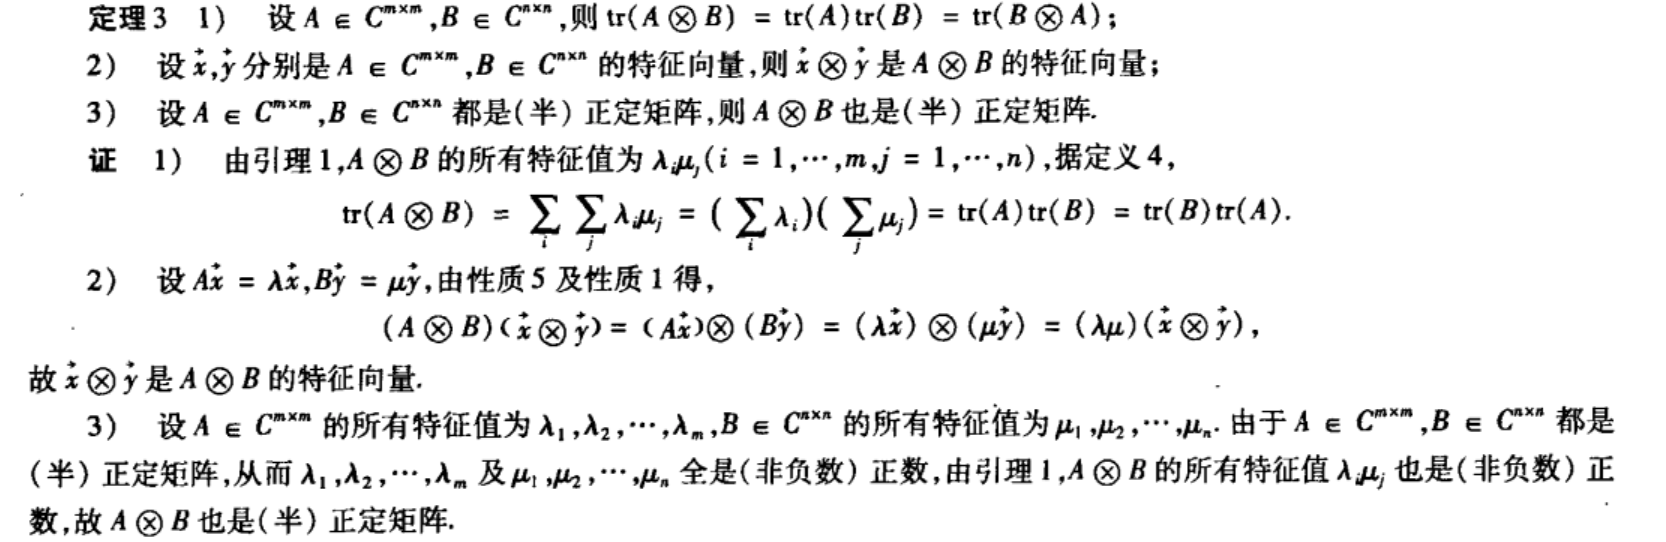
\includegraphics[scale=0.5]{1.png}
                % \caption{this is a figure demo}
                % \label{fig:pathdemo}
        \end{figure}
    \end{enumerate}
\end{solution}
%%%%%%%%%%%%%%%%%%%%%
\begin{problem}[SVM with Weighted Penalty]
    Consider the standard SVM optimization problem as follows (i.e., formula (6.35)in book),
    \[\min_{w,b,\xi_{i}}\frac{1}{2}\|w\|^2+C\sum_{i=1}^{m}\xi_i\]
    \[\mathrm{s.t.}~ y_i(w^Tx_i+b)\geq 1-\xi_i, \xi_i\geq 0,i=1,2,\cdots,m.\]
    Note that in (2.1), for positive and negative examples, the ”penalty” of the
    classification error in the objective function is the same. In the real scenario,
    the price of “punishment” is different for misclassifying positive and negative
    examples. For example, considering cancer diagnosis, misclassifying a person
    who actually has cancer as a healthy person, and misclassifying a healthy person
    as having cancer, the wrong influence and the cost should not be considered
    equivalent.\\
    Now, we want to apply $k > 0$ to the ”penalty” of the examples that were
    split in the positive case for the examples with negative classification results
    (i.e., false positive). For such scenario,
    \begin{enumerate}
        \item[(1)]  [10pts] Please give the corresponding SVM optimization problem;
        \item[(2)]  [15pts] Please give the corresponding dual problem and detailed derivation
            steps, especially such as KKT conditions.
    \end{enumerate}
\end{problem}

%\begin{remark}

%\end{remark}

\begin{solution}
    \begin{enumerate}
        \item[(1)]
            If misclassified case $y_i$ is positive, punishment is $\xi_i$.\\ However if misclassified case $y_i$ is negative, punishment is $k\xi_i$.\\
            So the SVM optimization problem will be
            \[\min_{w,b,\xi_{i}}\frac{1}{2}\|w\|^2+C\sum_{i=1}^{m}\frac{(k+1)-y_i(k-1)}{2}\xi_i\]
            \[\mathrm{s.t.}~ y_i(w^Tx_i+b)\geq 1-\xi_i, \xi_i\geq 0,i=1,2,\cdots,m.\]
        \item[(2)] Using the method of lagrange multipliers, we get that function:
            \[\frac{1}{2}\|w\|^2+C\sum_{i=1}^{m}\frac{(k+1)-y_i(k-1)}{2}\xi_i+\sum_{i=1}^m\alpha_{i}(1-\xi_i-y_i(w^Tx_i+b))-\sum_{i=1}^{m}\mu_i\xi_i\]
            The derivation of $w$ is \[w-\sum_{i=1}^{m}\alpha_iy_ix_i\]
            The derivation of $b$ is \[-\sum_{i=1}^{m}\alpha_iy_i\]
            The derivation of $\xi_i$ is \[C\frac{(k+1)-y_i(k-1)}{2}-\alpha_i-\mu_i\]
            That is to say
            \[
                \sum_{i=1}^{m}\alpha_iy_i=0
            \]
            \[
                \sum_{i=1}^{m}\alpha_iy_ix_i=w
            \]
            \[
                C\frac{(k+1)-y_i(k-1)}{2}=\alpha_i+\mu_i
            \]
            Then the dual problem is
            \[\max_{\alpha}\sum_{i=1}^{m}\alpha_i-\frac{1}{2}\sum_{i=1}^{m}\sum_{j=1}^{m}\alpha_i\alpha_jy_iy_jx_i^Tx_j\]
            \[\mathrm{s.t.}~ \sum_{i=1}^m\alpha_iy_i=0,\]
            \[0\leq \alpha_i\leq C\frac{(k+1)-y_i(k-1)}{2},i=1,2,\cdots,m.\]
            And the KKT conditions are
            \begin{enumerate}
                \item[1] raw posibility : $\alpha_i\geq 0,~ \mu_i\geq 0$
                \item[2] dual posibility : $y_i(w^Tx_i+b)-1+\xi_i\geq 0$
                \item[3] complementary slackness condition: $\xi_i\geq 0,~ \mu_i\xi_i=0$
                \item[4] Lagrangian stationarity: $\alpha_i(y_i(w^Tx_i+b)-1+\xi_{i})=0$
            \end{enumerate}
    \end{enumerate}
\end{solution}
%%%%%%%%%%%%%%%%%%%%%
\begin{problem}[Nearest Neighbor]
    Let $D = \{x_1, \cdots, x_n\}$ be a set of instances sampled completely at random from
    a $p$-dimensional unit ball $B$ centered at the origin,
    \[B=\{x:\|x\|^2\leq 1\}\subset\mathbb{R}^{p}\]
    Here, $\|x\| =\sqrt{\langle x,x\rangle}$ and $\langle\cdot,\cdot\rangle$ indicates the dot product of two vectors.\\
    In this assignment, we consider to find the nearest neighbor for the origin.
    That is, we define the shortest distance between the origin and $D$ as follows,
    \[d^*:=\min_{1\leq i\leq n}\|x_i\|.\]
    It can be seen that $d^∗$ is a random variable since $x_i$ , $\forall i, 1 \leq i \leq n$ are sampled completely at random.
    \begin{enumerate}
        \item[(1)] [5pts] Assume $p = 2$ and $t \in [0, 1]$, calculate $Pr(d^∗ \leq t)$, i.e., the cumulative distribution function (CDF) of random variable $d^∗$.
        \item[(2)] [10pts] Show the general formula of CDF of random variable $d^∗$ for $p \in\{1, 2, 3,\cdots \}$. You may need to use the volume formula of sphere with radius equals to $r$,
            \[V_{p}(r)=\frac{(r\sqrt{\pi})^p}{\Gamma(p/2+1)}.\]
            Here, $\Gamma(1/2)=\sqrt{\pi},\Gamma(1)=1,$ and $\Gamma(x+1)=x\Gamma(x),\forall x>0$. For $n\in\mathbb{N}^*$, $\Gamma(n+1)=n!$
        \item[(3)] [10pts] Calculate the median of the value of random variable $d^∗$, i.e., calculate the value of $t$ that satisfies $Pr(d^∗ \leq t) = 1/2$.
    \end{enumerate}
\end{problem}

%\begin{remark}

%\end{remark}

\begin{solution}
    \begin{enumerate}
        \item[(1)] for one ball, the distance shorter than $t$ is $\frac{\pi t^2}{\pi}=t^2$.\\
            Then we assume that all the distance is bigger than $t$, the probability is $(1-t^2)^n$.\\
            So $Pr(d^{*}\leq t)=1-(1-t^2)^{n}$.
        \item[(2)] for one ball, the distance shorter than $t$ is $\frac{Vp(t)}{Vp(1)}=\frac{(r\sqrt{\pi})^{t}}{\Gamma(t/2+1)}=t^p$.\\
            Then we assume that all the distance is bigger than $t$, the probability is $(1-t^p)^n$.\\
            So $Pr(d^{*}\leq t)=1-(1-t^p)^{n}$.
        \item[(3)] According to the probability we get from (2).\\
            $Pr(d^*\leq t)=1-(1-t^p)^n=\frac{1}{2}\Rightarrow 1-t^p=2^{-\frac{1}{n}}\Rightarrow t=(1-2^{-\frac{1}{n}})^{\frac{1}{p}}$
    \end{enumerate}
\end{solution}
%%%%%%%%%%%%%%%%%%%%%
\begin{problem}[Principal Component Analysis]
    \begin{enumerate}
        \item[(1)]  [5 pts] Please describe describe the similarities and differences between PCA and LDA.
        \item[(2)]  [10 pts] Consider 3 data points in the 2-d space: $(-1, 1), (0, 0), (1, 1)$, What is the first principal component? (Maybe you don’t really need to solve any SVD or eigenproblem to see this.)
        \item[(3)] [10 pts] If we projected the data into 1-d subspace, what are their new corrdinates?
    \end{enumerate}
\end{problem}

%\begin{remark}

%\end{remark}

\begin{solution}
    \begin{enumerate}
        \item[(1)]
            Similatiries:
            \begin{enumerate}
                \item[a.]
                    Both PCA and LDA are classical dimensionality reduction algorithms.
                \item[b.]
                    Both PCA and LDA assume that the data conforms to the gaussian distribution.
                \item[c.]
                    Both PCA and LDA make use of the idea of matrix eigendecomposition.
            \end{enumerate}
            Differences:
            \begin{enumerate}
                \item[a.]
                    PCA is unsupervised and LDA is supervised.
                \item[b.]
                    PCA is to remove the redundant dimension of the original data, while LDA is to select an optimal projection direction, so that the data of the same category are distributed compactness after projection, and the data of different categories are as far away from each other as possible.
                \item[c.]
                    At most, LDA can be reduced to k-1 dimension (k is the number of training samples, k-1 is because the mean of the last dimension can be represented by the mean of the previous k-1 dimension).
                \item[d.]
                    LDA may overfit the data.
            \end{enumerate}
        \item[(2)] As we can see $(1,0)$ is the first principal component.
        \item[(3)] Their new corrdinates are as follows:
            \[(-1,1)\to -1\]
            \[(0,0)\to 0\]
            \[(1,1)\to 1\]
    \end{enumerate}
\end{solution}
%%%%%%%%%%%%%%%%%%%%%
% \begin{problem}[TC 32.3-3]
% \end{problem}

%\begin{remark}

%\end{remark}

% \begin{solution}
%
% \end{solution}
%%%%%%%%%%%%%%%%%%%%
%\newpage
%%%%%%%%%%%%%%%%%%%%


%%%%%%%%%%%%%%%%%%%%%%%%%%%%%%%%%%%%%%%%%%%%%%%%%%%%%%%%%%%%%%%%
%                      Correction START!                       %
%%%%%%%%%%%%%%%%%%%%%%%%%%%%%%%%%%%%%%%%%%%%%%%%%%%%%%%%%%%%%%%%
\begincorrection
%%%%%%%%%%%%%%%%%%%%
%\begin{problem}[]

%\end{problem}

%\begin{cause}
%
%\end{cause}

%\begin{revision}

%\end{revision}
%%%%%%%%%%%%%%%%%%%%
%\newpage
%%%%%%%%%%%%%%%%%%%%


%%%%%%%%%%%%%%%%%%%%%%%%%%%%%%%%%%%%%%%%%%%%%%%%%%%%%%%%%%%%%%%%
%                       Feedback START!                        %
%%%%%%%%%%%%%%%%%%%%%%%%%%%%%%%%%%%%%%%%%%%%%%%%%%%%%%%%%%%%%%%%
\beginfb
%\begin{itemize}
%
%\end{itemize}


%%%%%%%%%%%%%%%%%%%%%%%%%%%%%%%%%%%%%%%%%%%%%%%%%%%%%%%%%%%%%%%%
%                        Homework END!                         %
%%%%%%%%%%%%%%%%%%%%%%%%%%%%%%%%%%%%%%%%%%%%%%%%%%%%%%%%%%%%%%%%
\end{document}

